% ------------------------------------------------------------------------------
% TYPO3 CMS 8.0 - What's New - Chapter "Introduction" (English Version)
%
% @author	Michael Schams <schams.net>
% @license	Creative Commons BY-NC-SA 3.0
% @link		http://typo3.org/download/release-notes/whats-new/
% @language	English
% ------------------------------------------------------------------------------
% LTXE-CHAPTER-UID:		cb43d098-7bf9a537-bf3817c0-53a0f29f
% LTXE-CHAPTER-NAME:	Introduction
% ------------------------------------------------------------------------------

\section{Introducción}
\begin{frame}[fragile]
	\frametitle{Introducción}

	\begin{center}\huge{Introducción}\end{center}
	\begin{center}\huge{\color{typo3darkgrey}\textbf{Los Hechos}}\end{center}

\end{frame}

% ------------------------------------------------------------------------------
% LTXE-SLIDE-START
% LTXE-SLIDE-UID:		c260d531-52d768d6-8db69386-64a8d24c
% LTXE-SLIDE-ORIGIN:	9e397afb-762f7061-0e0e0bd1-9836250e English
% LTXE-SLIDE-TITLE:		TYPO3 CMS 8.0 - The Facts
% ------------------------------------------------------------------------------
\begin{frame}[fragile]
	\frametitle{Introducción}
	\framesubtitle{TYPO3 CMS 8.0 - Los Hechos}

	\begin{itemize}
		\item Fecha de lanzamiento: 22 Marzo 2016
		\item Tipo de lanzamiento: Lanzamiento Sprint
		\item Eslogan: Enciendan sus motores
	\end{itemize}

	\begin{figure}
		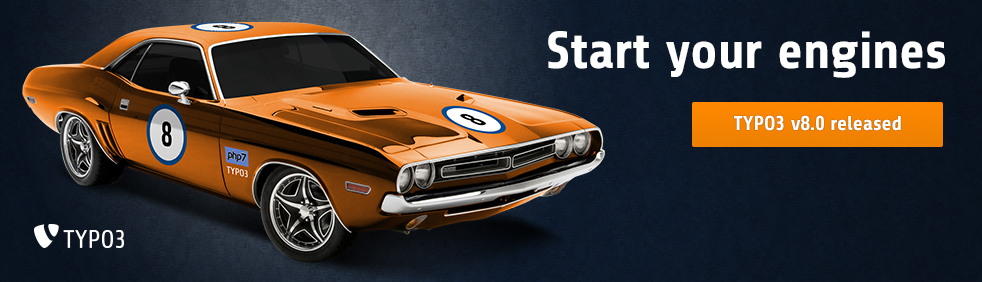
\includegraphics[width=0.95\linewidth]{Introduction/typo3cms80-banner.png}
	\end{figure}

\end{frame}

% ------------------------------------------------------------------------------
% LTXE-SLIDE-START
% LTXE-SLIDE-UID:		c5abfc13-2c328178-91c22d8b-4f62ccb3
% LTXE-SLIDE-ORIGIN:	737c8e9b-4ae60e26-6975ea72-21146dd0 English
% LTXE-SLIDE-TITLE:		System Requirements
% ------------------------------------------------------------------------------
\begin{frame}[fragile]
	\frametitle{Introducción}
	\framesubtitle{Requisitos del Sistema}

	\begin{itemize}
		\item PHP:\tabto{2.2cm}versión 7
		\item MySQL:\tabto{2.2cm}versión 5.5 to 5.7
		\item Disk space:\tabto{2.2cm}mín 200 MB
		\item Ajustes de PHP:

			\begin{itemize}
				\item \texttt{memory\_limit} >= 128M
				\item \texttt{max\_execution\_time} >= 240s
				\item \texttt{max\_input\_vars} >= 1500
				\item opción de compilación \texttt{-}\texttt{-disable-ipv6} \underline{NO} debe ser usada
			\end{itemize}

		\item El backend requiere Microsoft Internet Explorer 11 o posterior,
			Microsoft Edge, Google Chrome, Firefox, Safari o cualquier otro navegador
			moderno y compatible

	\end{itemize}

\end{frame}

% ------------------------------------------------------------------------------
% LTXE-SLIDE-START
% LTXE-SLIDE-UID:		7f92a9de-5632be64-1c97a810-b89d9ed5
% LTXE-SLIDE-ORIGIN:	90d2d3d1-f9d57661-dd01143b-10630416 English
% LTXE-SLIDE-TITLE:		Development And Release Timeline
% ------------------------------------------------------------------------------
\begin{frame}[fragile]
	\frametitle{Introducción}
	\framesubtitle{Línea de tiempo de Desarrollo y Lanzamiento}

	\begin{figure}
		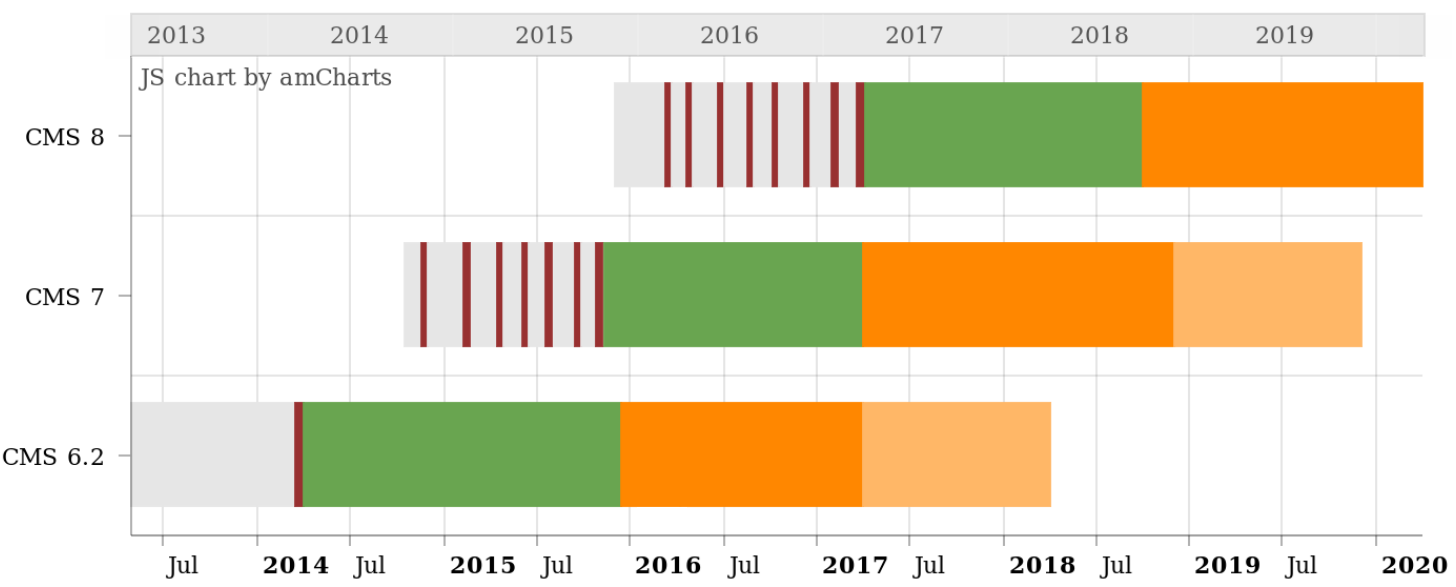
\includegraphics[width=1\linewidth]{Introduction/ReleaseAgenda.png}
	\end{figure}

\end{frame}

% ------------------------------------------------------------------------------
% LTXE-SLIDE-START
% LTXE-SLIDE-UID:		14b21f32-71f87e8a-497d00ed-17881b09
% LTXE-SLIDE-ORIGIN:	13e0fd6a-fa50d02d-c15c4af0-f3996926 English
% LTXE-SLIDE-TITLE:		TYPO3 CMS Roadmap
% ------------------------------------------------------------------------------
\begin{frame}[fragile]
	\frametitle{Introducción}
	\framesubtitle{Línea de lanzamiento de TYPO3 CMS}

	Fechas de lanzamiento y sus enfoques principales:

	\begin{itemize}

		\item
			\begingroup
				\color{typo3orange}
					v8.0 \tabto{1.1cm}22/Mar/2016\tabto{3.4cm}Añadiendo cosas de última hora
			\endgroup
		\item v8.1 \tabto{1.1cm}03/May/2016\tabto{3.4cm}Integración con la Nube
		\item v8.2 \tabto{1.1cm}05/Jul/2016\tabto{3.4cm}Editor de Texto Enriquecido
		\item v8.3 \tabto{1.1cm}30/Ago/2016\tabto{3.4cm}Edición del Frontend con Steroids
		\item v8.4 \tabto{1.1cm}18/Oct/2016\tabto{3.4cm}\textit{por determinar}
		\item v8.5 \tabto{1.1cm}20/Dic/2016\tabto{3.4cm}Soporte de Integrador
		\item v8.6 \tabto{1.1cm}14/Feb/2017\tabto{3.4cm}\textit{por determinar}
		\item v8.7 \tabto{1.1cm}04/Abr/2017\tabto{3.4cm}Preparación LTS

	\end{itemize}

	\smaller
		\url{https://typo3.org/typo3-cms/roadmap/}\newline
		\url{https://typo3.org/news/article/kicking-off-typo3-v8-development/}
	\normalsize

\end{frame}

% ------------------------------------------------------------------------------
% LTXE-SLIDE-START
% LTXE-SLIDE-UID:		da7bea11-b29b0a50-8b9a771d-2cdd9e6a
% LTXE-SLIDE-ORIGIN:	06c6100a-69216610-618bde63-bbdc4eef English
% LTXE-SLIDE-TITLE:		Installation
% ------------------------------------------------------------------------------
\begin{frame}[fragile]
	\frametitle{Introducción}
	\framesubtitle{Instalación}

	\begin{itemize}
		\item Procedimiento de instalación oficial bajo Linux/Mac OS X\newline
			(DocumentRoot por ejemplo \texttt{/var/www/site/htdocs}):
		\begin{lstlisting}
			$ cd /var/www/site
			$ wget --content-disposition get.typo3.org/8.0
			$ tar xzf typo3_src-8.0.0.tar.gz
			$ cd htdocs
			$ ln -s ../typo3_src-8.0.0 typo3_src
			$ ln -s typo3_src/index.php
			$ ln -s typo3_src/typo3
			$ touch FIRST_INSTALL
		\end{lstlisting}

		\item Enlaces simbólicos bajo Microsoft Windows:

			\begin{itemize}
				\item Use \texttt{junction} en Windows XP/2000
				\item Use \texttt{mklink} en Windows Vista y Windows 7
			\end{itemize}

	\end{itemize}
\end{frame}

% ------------------------------------------------------------------------------
% LTXE-SLIDE-START
% LTXE-SLIDE-UID:		1265dc7c-b541d01a-ec4c877a-91c17263
% LTXE-SLIDE-ORIGIN:	b878899c-e4b09ddf-4c0ea575-9e0900ad English
% LTXE-SLIDE-TITLE:		Upgrade to TYPO3 CMS 7
% ------------------------------------------------------------------------------
\begin{frame}[fragile]
	\frametitle{Introducción}
	\framesubtitle{Actualización a TYPO3 CMS 8.x}

	\begin{itemize}
		\item Actualizaciones sólo posibles desde TYPO3 CMS 7.6 LTS
		\item TYPO3 CMS < 7.6 LTS debe ser actualizado a TYPO3 CMS 7.6 LTS primero
	\end{itemize}

	\begin{itemize}

		\item Instrucciones de actualización:\newline
			\smaller\url{http://wiki.typo3.org/Upgrade#Upgrading_to_8.0}\normalsize
		\item Guía oficial de TYPO3 "Instalación y Actualización de TYPO3":
			\smaller\url{http://docs.typo3.org/typo3cms/InstallationGuide}\normalsize
		\item Enfoque general:
			\begin{itemize}
				\item Comprobar requisitos mínimos del sistema \small(PHP, MySQL, etc.)
				\item Revisar \textbf{deprecation\_*.log} en instancia antigua de TYPO3
				\item Actualizar todas las extensiones a la última versión
				\item Desplegar fuentes nuevas y ejecutar Herramienta de Instalación -> Asistente de Actualización
				\item Revisar el módulo de inicio para usuarios backend (opcionalmente)
			\end{itemize}
	\end{itemize}

\end{frame}

% ------------------------------------------------------------------------------

% ------------------------------------------------------------------------------
% LTXE-SLIDE-START
% LTXE-SLIDE-UID:		79d5afd3-3065aa6e-bae12afb-cf77a9c1
% LTXE-SLIDE-ORIGIN:	e4b09ddf-4c0ea575-9e0900ad-b878899c English
% LTXE-SLIDE-TITLE:		PHP Version 7
% ------------------------------------------------------------------------------
\begin{frame}[fragile]
	\frametitle{Introducción}
	\framesubtitle{PHP Versión 7}

	\begin{itemize}

		\item PHP 7.0 es el requisito mínimo para TYPO3 CMS 8.x
		\item TYPO3 soportará posteriores lanzamientos de PHP 7 cuando aparezcan
		\item Este aumento de versión proporciona un significativo aumento de rendimiento de todo el sistema

		\item No sólo los editores del backend notarán una interfaz más fluida, sino que el
			tiempo al completo para una llamada de página cacheada en el frontend no supera los
			7 milisegundos ahora, que es aproximadamente el 40\% más rápido si lo comparamos a ejecutar
			la misma página web con PHP versión 5.5

		\item También comenzamos a usar nuevas características de esta versión de PHP, por ejemplo
			los generadores seguros criptográficamente pseudo-aleatorios están ya en uso activo

	\end{itemize}

\end{frame}

% ------------------------------------------------------------------------------
